\documentclass[12pt]{article}
\usepackage{graphicx}
\usepackage{subcaption}
\usepackage{mwe}
\usepackage{amsmath}
\usepackage{mathtools}
\usepackage[]{mcode}
%\usepackage{lingmacros}
%\usepackage{tree-dvips}
%\usepackage{blindtext}
%\usepackage[utf8]{inputenc}

\newcommand{\norm}[1]{\left\lVert#1\right\rVert}
\newcommand{\abs}[1]{\left|#1\right|}

\begin{document}

\title{CMSC 426 - P4}
\author{Gudjon Einar Magnusson}

\maketitle

\section{Introduction}

The goal of this project is to track the precise boundary of an object of interest through a sequence of frames. The object, camera and background may or may not be moving. The only assumption is that the precise shape and location of the object is given for the first frame and that the object will only make small movements from one frame to the next.

\section{Select the Object of Interest}

To be able to track an object of interest, we first need to know what that object is. To do this the boundary of the object needs to be marked on the first frame. This is done using the \textit{roipoly} Matlab function. It allows the user to draw an arbitrary polygon on top of an image and returns that polygon as a binary mask. Figure \ref{fig_roi1} shows an example of how the polygon is drawn to track a turtle in a video.

\begin{figure}
	\centering
    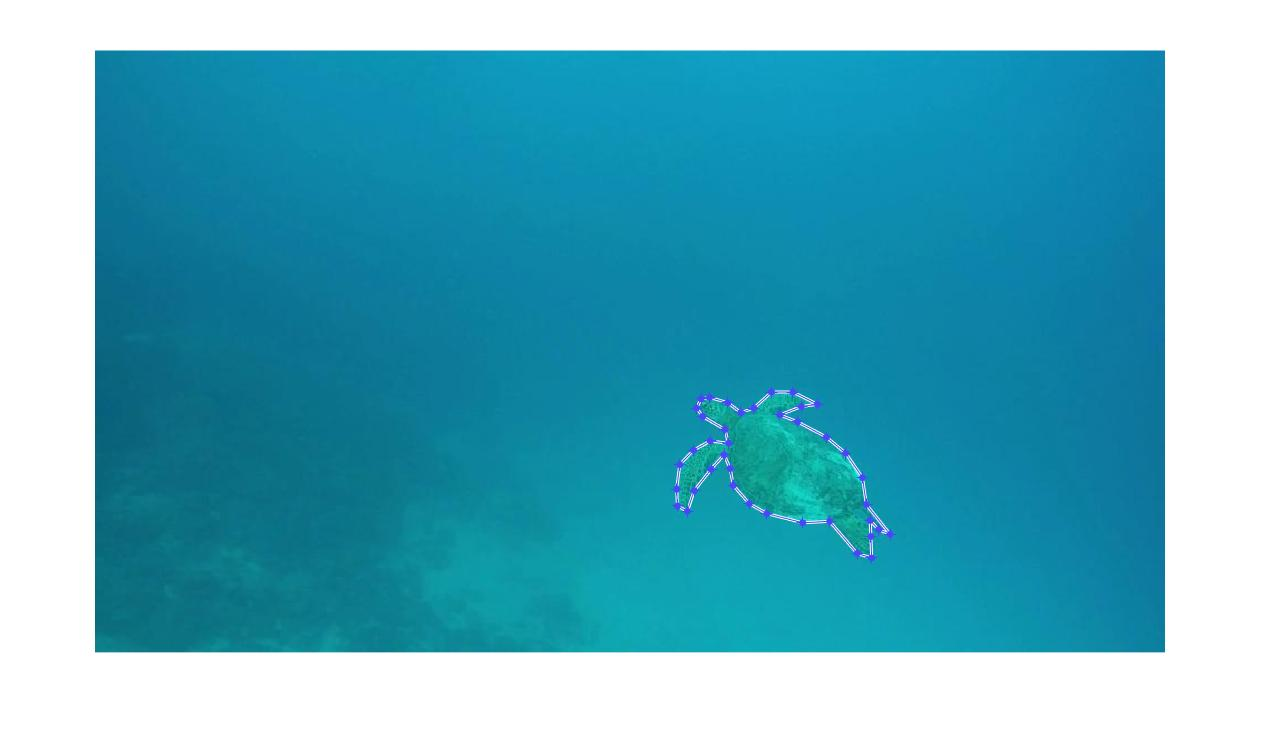
\includegraphics[width=0.6\linewidth]{img/video1_mask1}
    \caption{Capturing the region of interest using a hand drawn polygon}
    \label{fig_roi1}
\end{figure}

The user supplied mask does not need to be pixel perfect, it just needs to be good enough to supply sufficient examples of foreground and background pixels. The mask is used to generate a classifier that is then used to refine the mask.


\section{Color classifier}

A color classifier is generated taking the mean of all the pixels inside the foreground mask and the mean of all pixels on the outside. This gives two class centroids, $\mu_{FG}$ and $\mu_{BG}$. Each pixel $x_i$ can now be classified using the formula 

\[
1 - \frac{\norm{x_i - \mu_{FG}}}{\norm{x_i - \mu_{FG}}+\norm{x_i - \mu_{BG}}}
\]

This gives a new gray scale mask where the intensity of each pixel represents the probability that the pixel belongs to the foreground.

\section{Windows}



Split the object region into a bunch of overlapping windows. For each window we generate foreground and background classifier.



\end{document}